\chapter{Design and implementation}
This chapter contains the design of MultiChain and how it was implemented.
We will describe how MultiChain is part of Tribler and its main pillar of design.
The contents of blocks are presented and how they form chains in MultiChain.
We will cover the creation of blocks and the multiple implications of the chosen design.
Additional pheripheral systems that work with MultiChain are also explained.

\section{MultiChain Community}
Tribler uses communities to add functionalities to peers.
A peer loads in a community and this community provides a set of messages and endpoints for other peers.
The community can communicate with the endpoints of other peers as well and send a message to these endpoint.
Other peers are automatically discovered using Dispersy.
Examples of a community are the TunnelCommunity that adds functionality to download anonymously\cite{Plak-anonymous}
or the AllChannelCommunity to distribute torrent files.
The designed system will be implemented by adding a new community to Tribler.

The MultiChain community can be run standalone,
but its main use is to integrate with Tribler and track up and download for torrents.
It will replace the current reputation system Bartercast in the future.
\section{Abandoning full transaction history distribution}
One of the main pillars of the design is to have a transaction history for every peer.
This is in contrast to not distribute a common, full transaction history containing the transactions of every peer.
For example used in the design of the blockchain of Bitcoins, discussed in section \ref{sect:bitcoin}.
The reasoning behind the idea to abandon is that a common, full truth
will become the bottleneck in the system.
This will limit the amount of interactions that can be processed
or will limit the participiation of less powerfull machines.

The reason for the limitation is that every interactions will have to be distributed to every peer in the network.
Every transaction has to be processed by every node at the cost of bandwidth, compute power and storage.
The cost might be very limited for a single transaction,
but with greater scale these cost will add up.
The amount of these three resources is limited and will limit the amount of transactions that can be processed.
This problem can be seen to affect Bitcoins and has been demonstrated in section \ref{bitcoin-limit-size}.

Every node has its own transaction history and only needs the transaction history of its peers it interacts with.
The amount of bandwidth, compute power and storage is limited to the minimal needed amount
that is needed to process only the relevant transactions.
This should allow low-powered devices to keep participating when they only have a low volume of transactions.
It also allows higher volumes of transactions in the system as a whole.
\section{Transactions}
A peer will have transactions with other peers in the network.
The peer will want to have an increase in his reputation and have a transaction be created.
The transaction contains the information about how much data was uploaded and downloaded between the peers
and their total upload and download amounts.

The transaction will be encapsulated inside a single block.
A block contains both public keys of the peers,
so it is possible to see between which peers the transaction is.
Both peers sign the block to acknowledge that the transaction has happened.
Every block only contains one transaction.

The blocks are linked to previous blocks by adding the hashes of the previous blocks of both peers.
This creates a directed acyclic graph of blocks.
A chain can be identified within this graph for every peer.
This chain contains every transaction of a peer.

An example of three blocks can be seen in Figure \ref{fig:chain-example}.
The arrows denote the corresponding hash or signature.
In this example the first block is between peer B and C.
The block contains hashes to the previous blocks of both B and C
and can be seen by the outward arrows.
Inside the block it can be seen what part peer B and C signs by the boxes.
The whole block is not signed by both parties.
The reason for this is explained in section \ref{design:block_creation}.

In the example both peer B and C also conduct a transaction with another peer, A and D respectively.
This creates two new blocks and are chained to the block between B and C by adding the previous hash to the new blocks.
The new blocks also contains the previous hashes of A and D
and chain the new block to previous blocks of A and D.

\begin{figure}
	\centerline{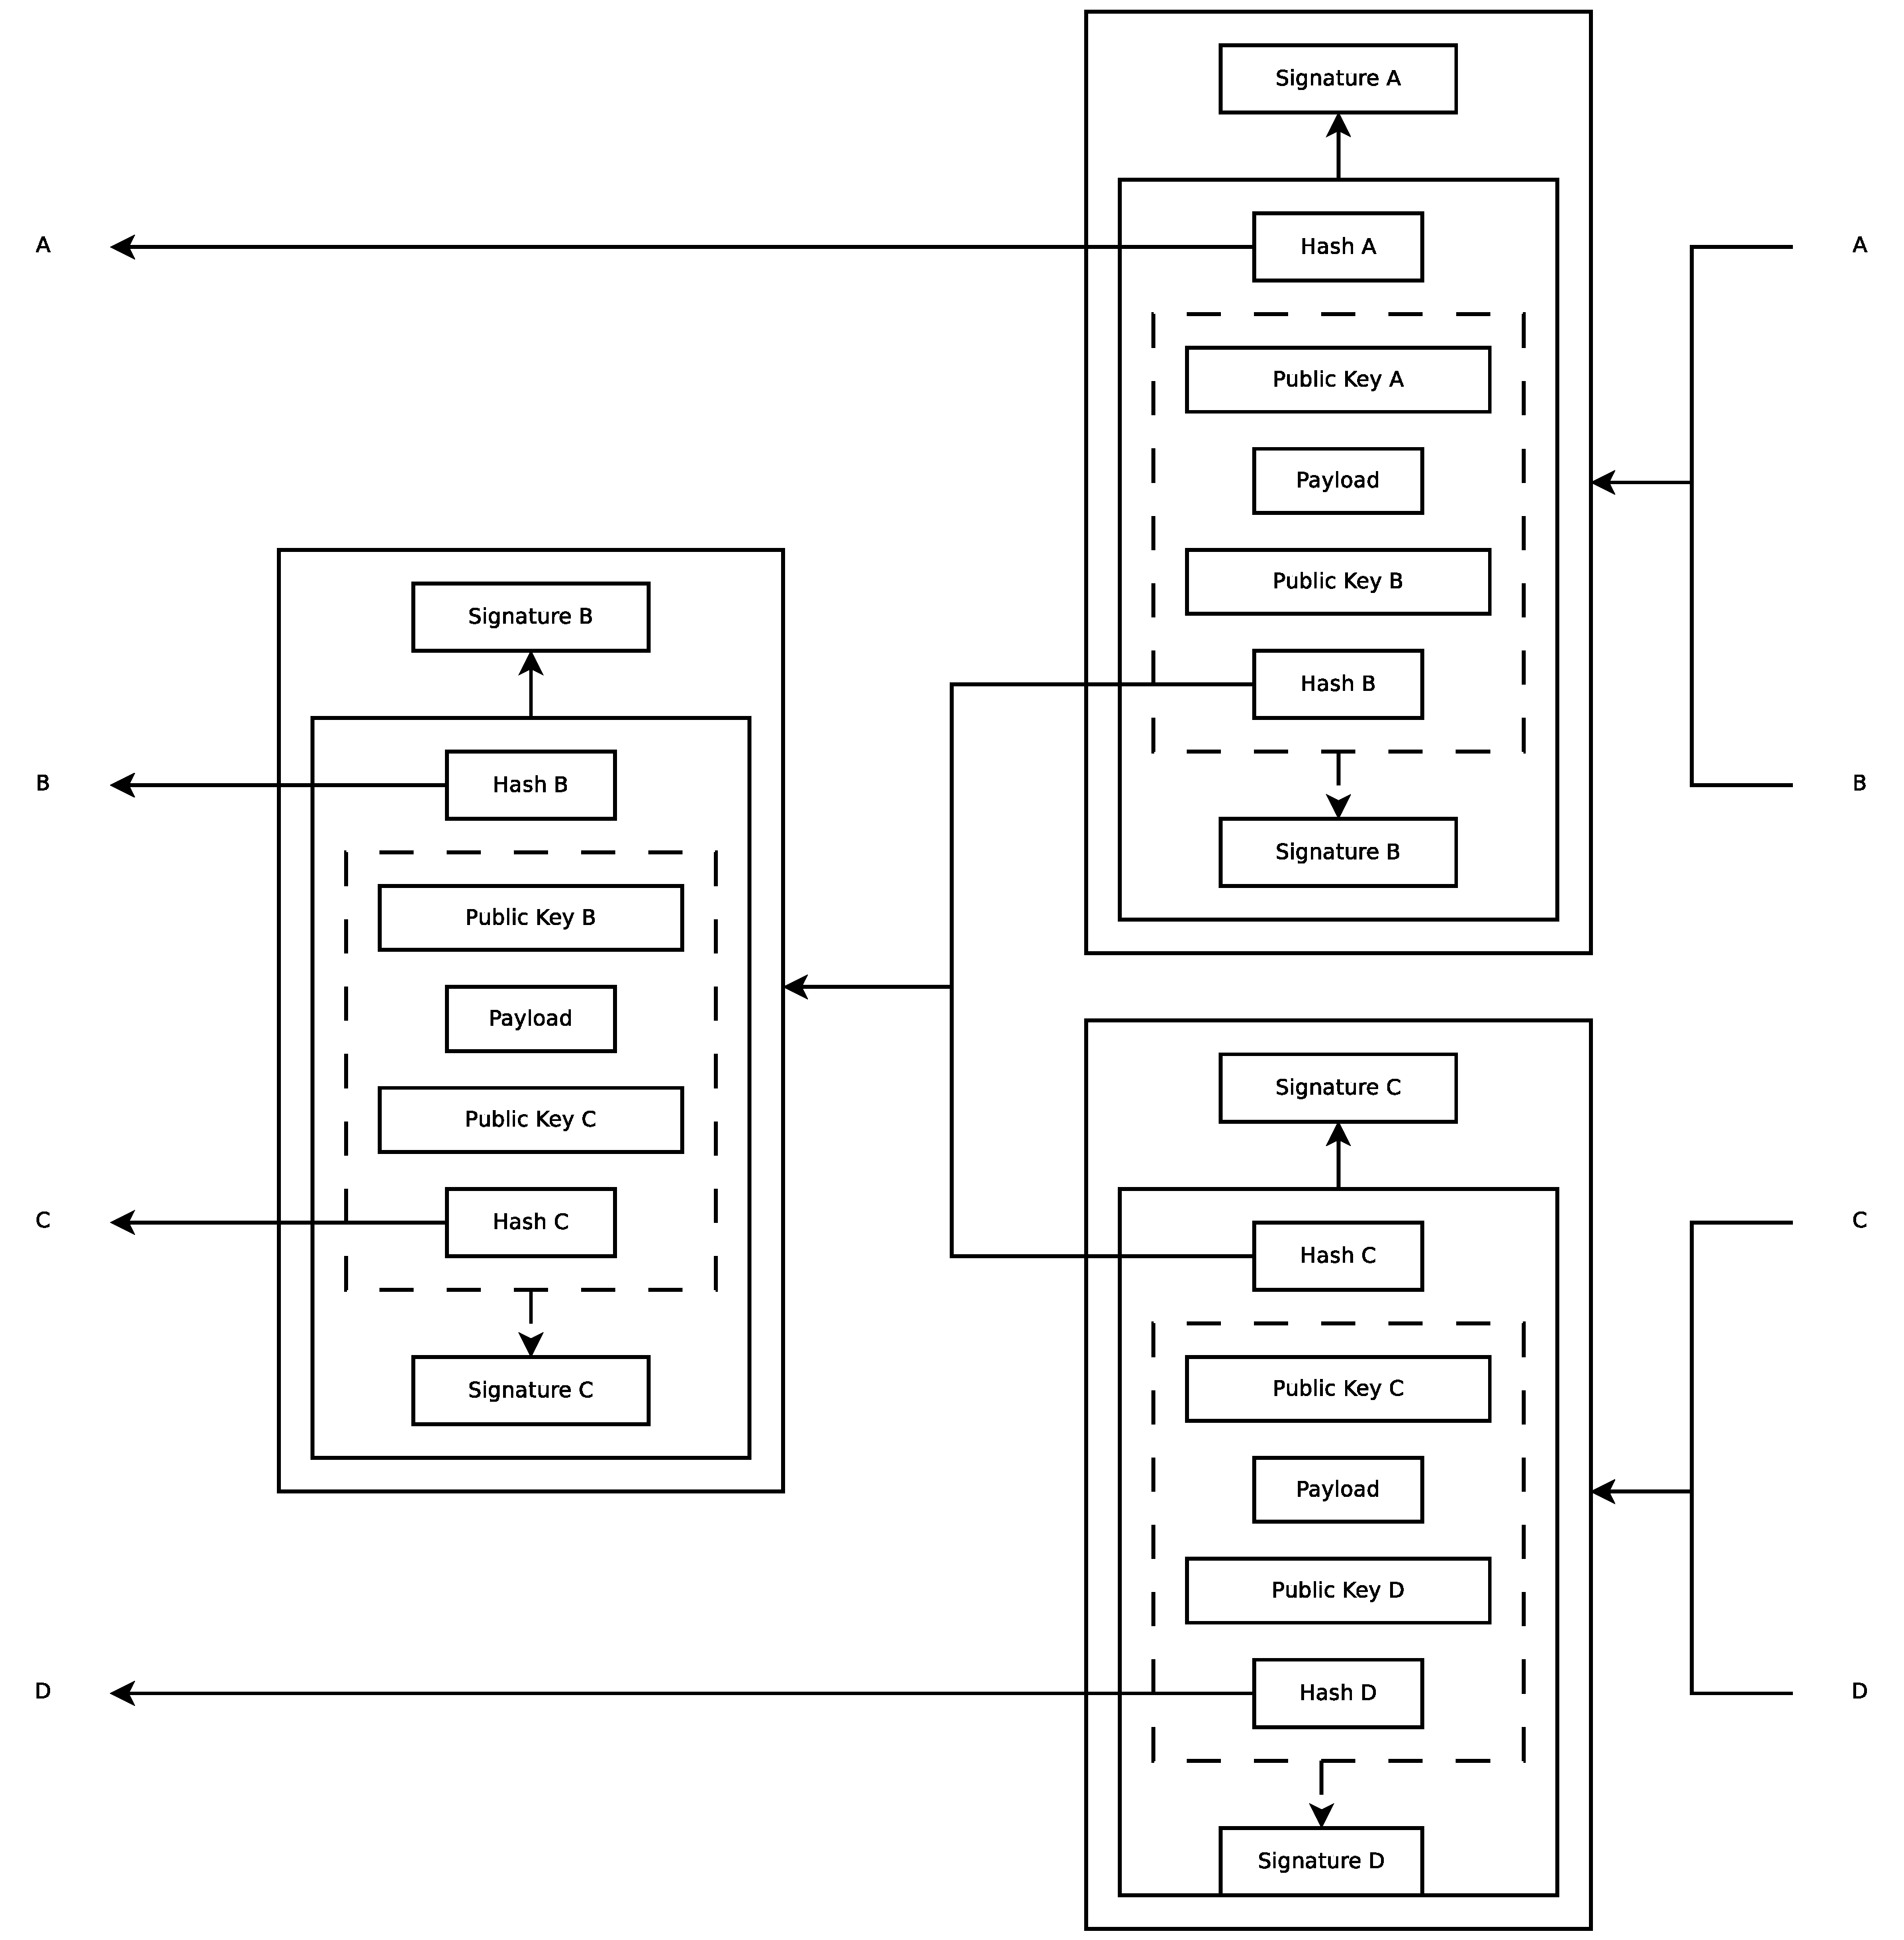
\includegraphics[scale=0.3]{design/figs/chain.eps}}
	\caption{Example of three blocks in the chain.}
	\label{fig:chain-example}
\end{figure}
\subsection{Exchanging signatures}
Two peers in a network will create their blocks together without having to rely on a third party.
Between the peers one is uploading to the other.
The uploader is traditionally called the seeder in BitTorrent and the receiver of this data the downloader~\cite{Cohen-bittorrent}.
The seeder will initiate the block creation.\,
co the seeder can decide how altruistic it wants to be towards the downloader regarding its collaboration.
We will explain how the block creation protocol works.
A sequence diagram can be seen in Figure \ref{fig:exchange-new-sequence}.

\begin{figure}[tpb]
\centering
\subfigure[Sequence diagram for block creation.]{
\centerline{\includegraphics[scale=0.3]{design/figs/exchange_new.eps}}
\label{fig:exchange-new-sequence}
}

\subfigure[Data added by peer A and B for a new block.]{
	\centerline{\includegraphics[scale=0.3]{design/figs/packet_creation.eps}}
\label{fig:packet-creation}
}
\caption{Exchanging data with our cleaner design in Dispersy.}
\label{fig:block-creation-new}
\end{figure}

The seeder, A, will create a packet that will be sent to the downloader, B.
A will add to this packet the data uploaded and downloaded data between the peers
that has not yet been added to the MultiChain.
It will add these amounts to its total uploaded and downloaded data
and add these total amounts aswell to the packet.
Finally, it adds the public keys of both peers and its own hash pointer to the packet.
This packet is signed using its private key and sent to the downloader.
The data that A adds can be seen in Figure \ref{fig:packet-creation}.

B will receive this packet and check if the amounts are correct, if the signature is correct,
and if A has not used the previous hash before.
If this is all correct,
then B will add the amounts of uploaded and downloaded data to its own total amounts.
The data contained in the previous packet, the total amounts of B and the hash of the previous block is
inserted into a new packet.
This packet is signed by the private key of B and sent back to A.
The data that B adds can be seen in Figure \ref{fig:packet-creation}.

Both parties now have the data of the block and can add this to their chain and continue forward.
A does this upon receival of the block.
B does this immediatly after sending the return packet to A.
At this point a new block is created.

\subsubsection{Integrating with Dispersy}
\begin{figure}[!h]
\centering
\subfigure[Sequence diagram for block creation.]{
\centerline{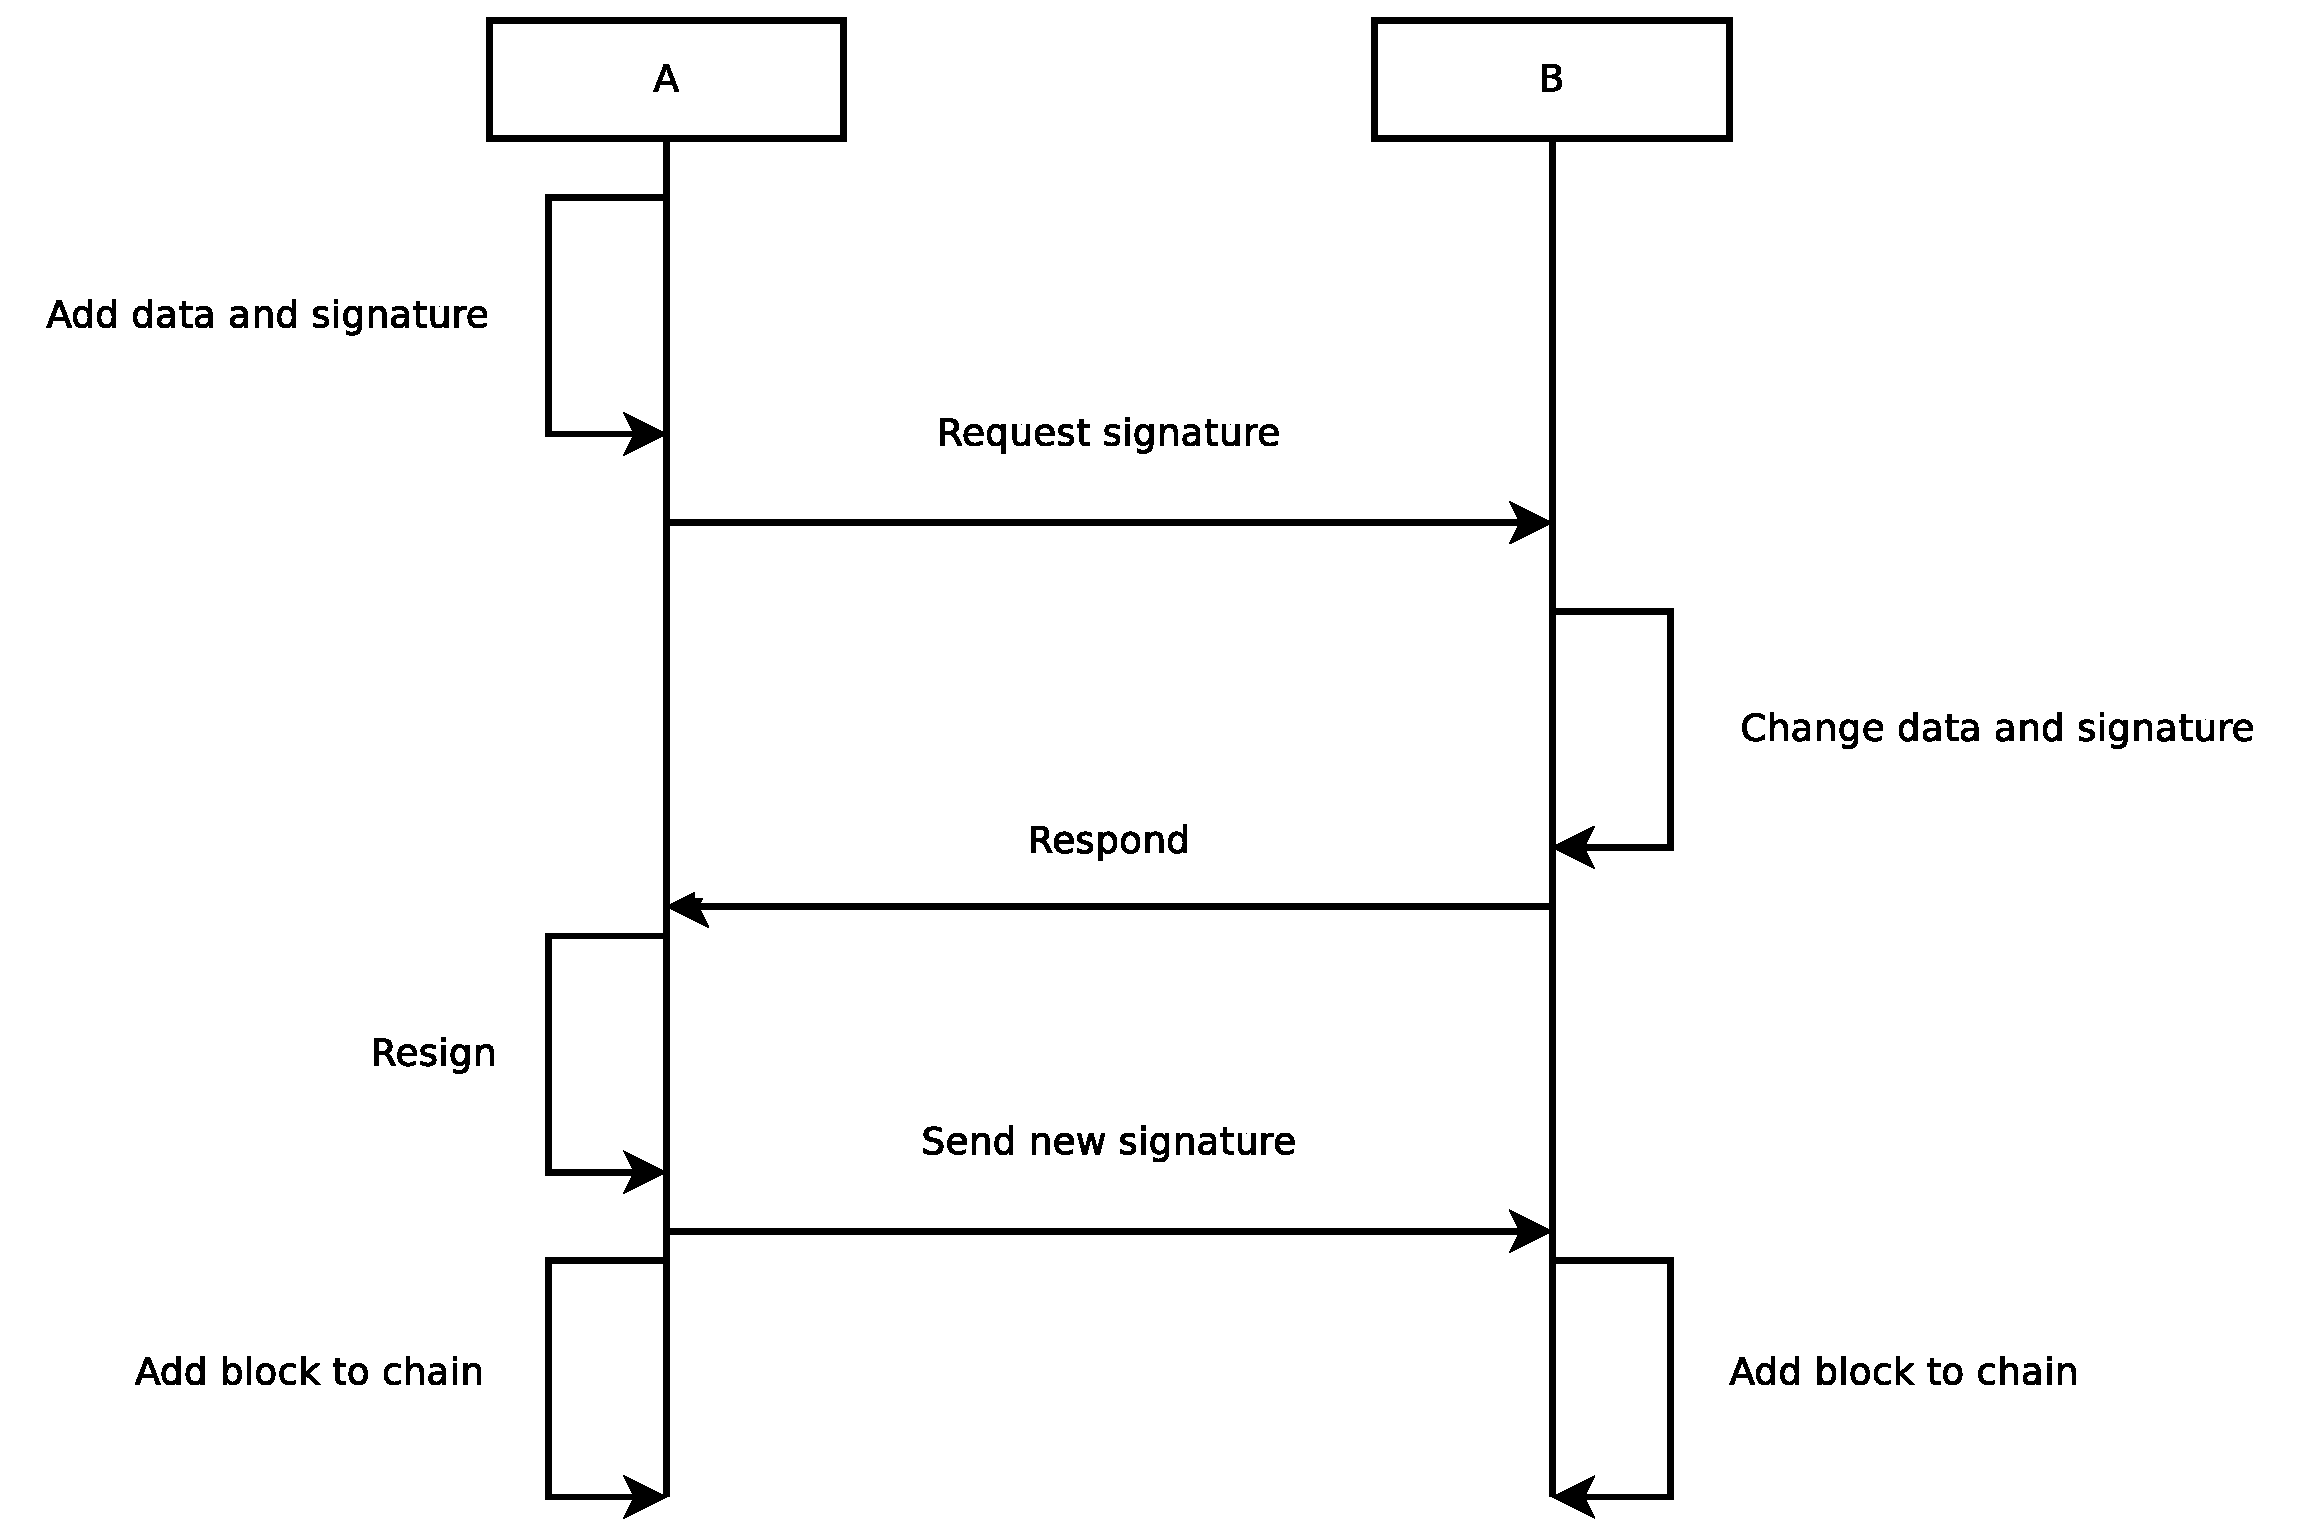
\includegraphics[scale=0.3]{design/figs/exchange_old.eps}}
\label{fig:exchange-old-sequence}
}

\subfigure[Data added by peer A and B for a new block.]{
	\centerline{\includegraphics[scale=0.3]{design/figs/signature_old.eps}}
    \label{fig:payload-signature-old}
}
\caption{Exchanging data for block creation using the old design in Dispersy.}
\label{fig:block-creation-old}
\end{figure}
Within Dispersy functionality was already build to create a message, sign the message
and request multiple nodes to also provide their signature on this message.
This existing functionality could be used by MultiChain to exchange signatures
between A and B for the creation of a new block.

A would initiate a message, insert its data into this message, sign the message, and send this message to B.
The functionality would allow B to accept the message and provide its signature or
modify the message and then provide its signature.
Only B knows the hash of its head node, and the total up and total download metrics.
So B will always modify the message and insert its own data in the message.
But this would invalidate the signature of A,
because the signature of A was also placed on the empty part of the message where the data of B is inserted.
The contents of the message and who signs what can be seen in Figure \ref{fig:payload-signature-old}.

After B returns the message,
A would have to resign the message.
But B also needs this valid signature from A before it can add the block to its own chain.
So A would need to send a third message to with the new, valid signature back to B.
A sequence diagram can be seen in Figure \ref{fig:exchange-old-sequence} of how it would work in Dispersy.
Functionality was added to Dispersy that allows to append data in a signature request.
This allows the full signature exchange to be achieved within two messages.
\section{Atomic operations on the chain}
\label{sect:deadlock}
In a chain, only a single block of a peer is allowed to point to a previous block.
No side branches are allowed.
A peer cannot have multiple blocks belonging to him all pointing to the same previous block.
As this is a potential attack as described in section \ref{sect:branch}.
The chain of a peer can only be moved forward by a single block at any time.
Only after a new block is created, will the new hash available to be used in the next block.

To ensure this happens correctly, the MultiChain community contains mutual exclusive code
that excludes any new operations on the chain if an operation is already pending.
The mutual exclusion is achieved by having to acquire an atomic token to allow to perform an operation on the code.
The MultiChain community will receive incoming signature requests
or requests by other parts of Tribler to send out an outgoing signature request.
The community will decline this request if the token is not available
returns execution to other parts of Tribler.
The token can be unavailable while waiting on another peer in the network to finish responding to a signature request.

When a MultiChain peer has a pending signature request,
then the peer itself will not respond to incoming signature requests from other peers.
These peers themselves will also not respond as they have a pending signature request.
This can create a circular dependency on the availability of the token.
If two peers send a request to each other at the same time, they will wait on each other.
This could result in a deadlock.

MultiChain prevents this deadlock to occur by allowing a transaction to fail
as explained in section \ref{des:halfsigned}.
If MultiChain gets into this potential deadlock one of the peers will eventually time out of their own signature request
and process the incoming request resolving the circular dependency.
The deadlock is recovered and both peers can continue operation.
This situation has occured during experimentation and it is explained in section \ref{sect:deadlock-exp}.
It is shown that MultiChain correctly recovers the potential deadlock.
A potential attack vector is explained in \ref{sect:denial}


\section{Block persistence}
The blocks in the chain have to be persisted to be usable over a prolonged time.
A persistence layer is added to the MultiChain community
that provides all functionality to persist blocks and query blocks.
This layer extends and uses functionality of the Database class in Dispersy.
An overview of the layering in the software architecture can be seen in Figure \ref{fig:persistence-layer}.

\begin{figure}
	\centerline{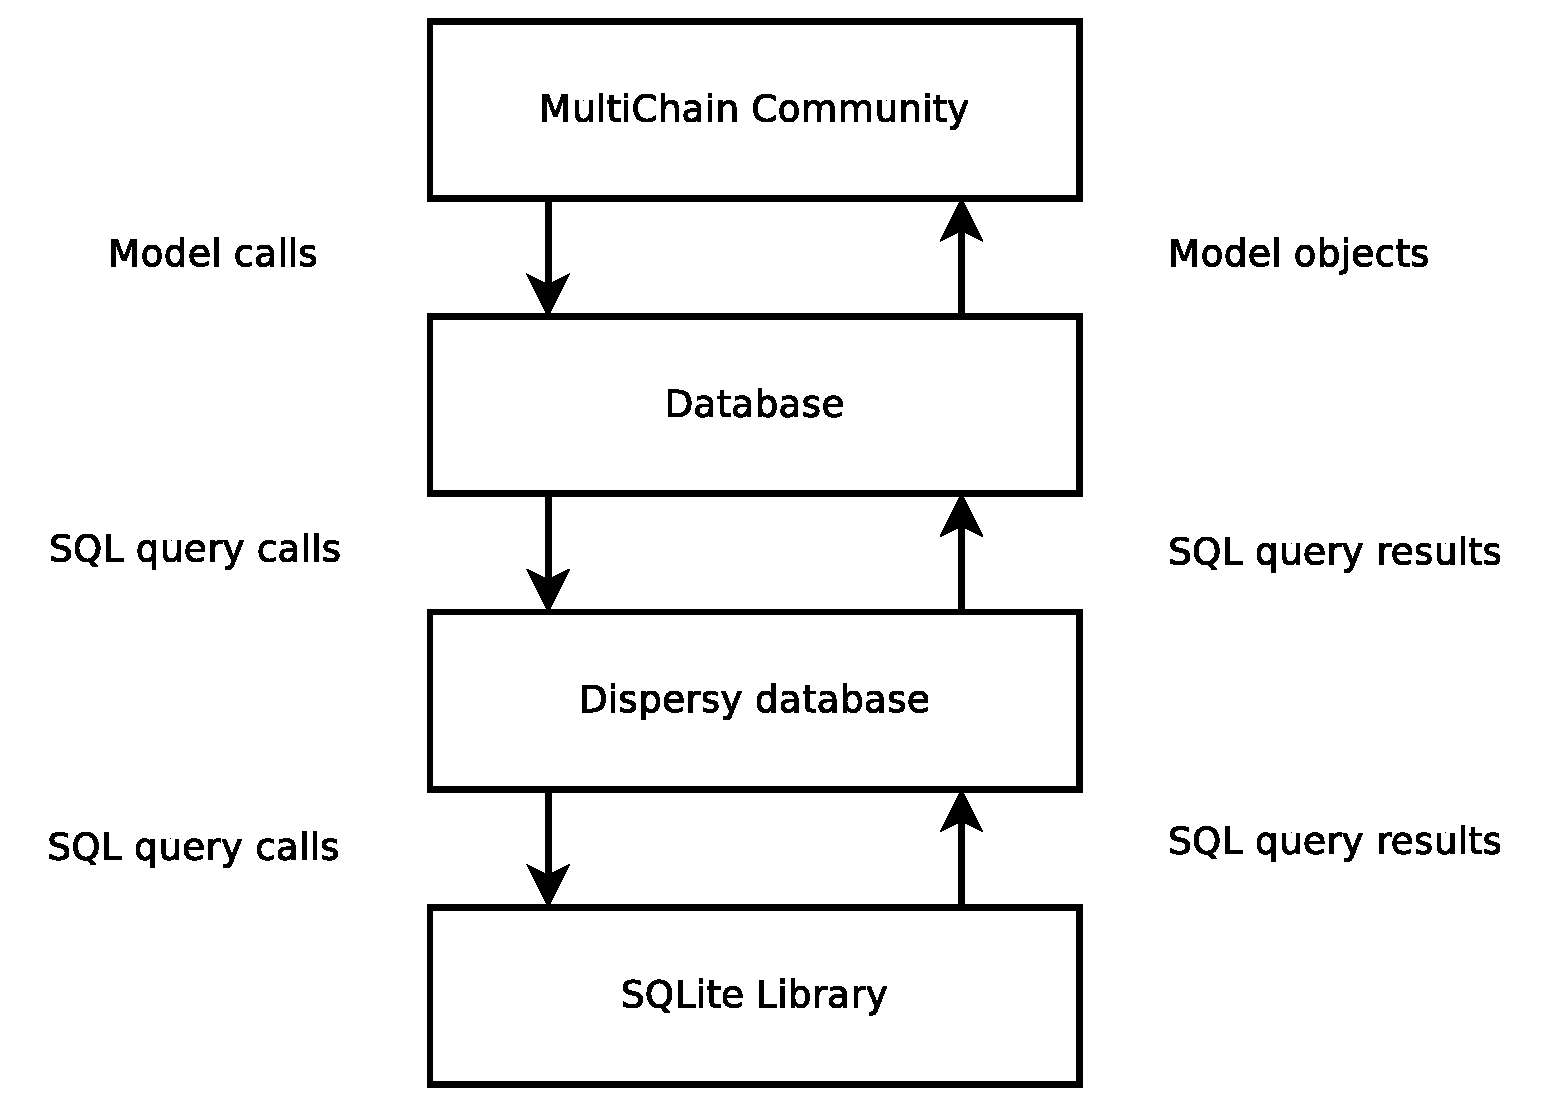
\includegraphics[scale=0.3]{design/figs/persistence-layer.eps}}
	\caption{Persistence layering in the software architecture}
	\label{fig:persistence-layer}
\end{figure}

The MultiChain Community calls functions in the persistence layer that have implicit knowledge about the model.
The Persistence layer formats SQL queries and passes these to the Dispersy layer.
The Dispersy layer performs several sanitation checks and passes these queries to the SQLite Library.
The SQLite Library and Dispersy layer both return the result of the SQL query.
These results are transformed by the Persistence layer into objects of the model usable by the MultiChain Community.

The only information that is saved are blocks.
The information all fits within one table.
A single block is saved as a single record called a row in a relation database.
Every attribute of a block is a single column in the row.
All attributes are saved directly into the database,
except for the public keys.
These public keys are hashed and these hashes are used as an identifier, called mid, in Dispersy.
The public keys are already saved in the Dispersy database.
When a block is retrieved from the database the public key is retrieved from Dispersy using the mid.

Every attribute is queryable in the database.
A public key can be converted to mid and is searched this way.
Every attribute is queryable to make the system  extensible
and usable when the next incremental steps are implemented.
It is presently unknown what information precisly will be needed,
so every information is now made available for the future.

\subsection{Dispersy database}
Dispersy keeps track of information on its own.
A record is kept of any message that can be retrieved using a message id.
The message is saved in a converted format and will be decoded when the message is retrieved.

Instead of storing information in a separate database,
the information could have been retrieved from the Dispersy database.
But the Dispersy database is not queryable.
All the information is stored in a converted format
that prevents queries to search the message for its contents.
For this reason, the dispersy database is not used and a separate database is used.

A future, possible improvement to Dispersy would be to save messages queryable in its database.
This would eliminate the current need for separate databases that contain aggregrated information.
The information is stored in two places within Tribler and this could be eliminated.
It would reduce the disk footprint and the amount of read/write transactions
as only one database would have to be maintained.
The I/O ineractions are a problem according to Tribler maintainers.

\section{Integration with Tribler}
The MultiChain community can be run standalone,
but its main use is to integrate with Tribler and track up and download for torrents.
It will replace the current reputation system Bartercast in the future.

For integration a scheduler is implemented between the MultiChain community
and the community that handles the anonymous download.
For additional detail on the anonymous download communities see \cite{Plak-anonymous}\cite{ruigrok-anonymous}.
The scheduler tracks session up and download amounts and schedules a block to be created,
when the amount of uploaded bytes is above a certain threshold.
The scheduler currently only tracks traffic of anonymous downloads.
Bartercast is not yet removed and
currently MultiChain runs together with Bartercast untill MultiChain fully replaces Bartercast.

The scheduler should be expanded in the future to schedule blocks in a more sophisticated way.
The functionality of the scheduler is very limited and is missing basic functionality.
The most important improvement that should be introduced is the punishment of not signing blocks.
Currently, nodes can deny to have their behaviour tracked.
The next improvement is to actually determine the level of cooperation a node receives based upon their previous behaviour.
The actual decision making based upon past behaviour is not part of the thesis.
\section{Crawler}
A crawler was implemented that visits other nodes and request the full chain of that node.
The crawler was used for the experiments and
is a first step in a more sophisticated crawler that will help to solve the known vulnerabilities.
These vulnerabilities will be described in chapter \ref{problems}.

\subsection{Recursively request blocks}
Dispersy provides a list of other nodes that were recently found
and can report when the node itself is found by an other node.
Both are sources of destinations nodes that the crawler will visit
and request the chain from.

The crawler will first request from a node the block with sequence number $-1$.
This denotes that he wants the latest block in his chain.
The node returns this block to the crawler.
The crawler will persist the block if it is not yet know.

The newly retrieved block is chained to two blocks with the previous hashes.
The crawler will check if these blocks are present in the database.
If any block is not present,
then the crawler will request that particulair block if the node is known in Dispersy.
If the node is not known, the block is ignored.
This is done recursively untill the crawler reaches the genesis block of the chain.
In this fashion a breadth first search is implemented for any unknown block
that is chained in chronologically before the latest block.

\begin{figure}
	\centerline{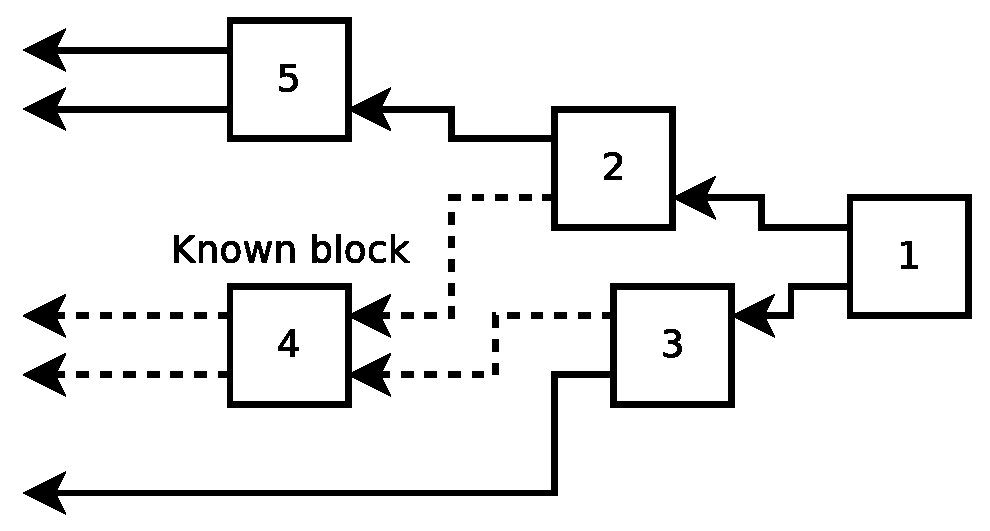
\includegraphics[scale=0.3]{design/figs/crawler.eps}}
	\caption{Example of the crawler looking for unknown blocks.}
	\label{fig:crawler-example}
\end{figure}

An example can be seen in Figure \ref{fig:crawler-example}.
In this example the line arrows denote paths that the crawler follows
and dotted lines are paths that the crawler ignores.
Block 4 is already known by the crawler.
Block 1 is retrieved by the crawler and the crawler sees hash links to block 2 and 3.
These are retrieved and the block finds links to block 4 and 5.
Because block 4 is already known, block 4 is ignored.
Only block 5 is retrieved.
The crawler follows the links further outside the displayed example.

\subsection{Improvements}
The crawler is a first, simple step towards a more sophisticated crawler.
Tribler has implemented already more sophisticated crawlers for Bartercast
and these techniques can be reused for the MultiChain crawler.
For example bloom filters can be used in conjunction with the knowledge
that every record is a part of the chain to quickly request multiple blocks\cite{broder-bloomfilter}\cite{logiotatidis-splash}.
Blocks could also be send in a more efficient way by sending multiple blocks per message.
Lastly an obvious improvement is to also crawl and retrieve blocks from other nodes present in a node.
This is currently not yet implemented.



\section{Anonymity}
Tribler has made an effort in providing a way for users to download anonymously\cite{Plak-anonymous}\cite{ruigrok-anonymous}.
There is anonymity in the contents of what is downloaded, not in how much is downloaded.
MultiChain obviously cannot break this anonymity to be usuable for anonymous downloads.
The introduction of anonymity increases the necessity of a good reputation system as more data has to be transferred.

MultiChain only interacts with peers that are directly downloaded from or uploaded to.
With these peers blocks are created and transferred.
So anonymity is not broken by MultiChain.
An attacker could already analyse network traffic between these peers
and conclude they are downloading and uploading to each other.
But Tribler does not guarantee anonymity for this.
So MultiChain does not break anonymity with its interactions with peers.

A block only transcribe the amount of data that has been transferred between peers.
The content of the actual data is not transcribed.
The block also does not leak information of how big a single, individual transfer is between peers.
The amounts are aggregrated over all transfers.
The blocks also does not break the anonymity.
Network analysis can already measure the total amount of data transferred.
So the design and implementation of MultiChain does not break anonymity already guaranteed by Tribler.

But MultiChain does make network analysis easier as measurement points between every node do not have to be introduced.
The chain of every node can be requested.k
The chain contains the data of every transaction of a peer and can be used to analyse the network.
